\documentclass{article}
\usepackage[utf8]{inputenc}
\usepackage[T1]{fontenc}
\usepackage{amsmath}
\usepackage{makeidx}
\usepackage{graphicx}
\usepackage{float}
\usepackage[width=17.00cm, height=24.00cm]{geometry}
\usepackage[polish]{babel}
\usepackage{fixltx2e}
\usepackage{color}
\usepackage{algpseudocode}% http://ctan.org/pkg/algorithmicx
\algtext*{EndWhile}% Remove "end while" text
\algtext*{EndIf}% Remove "end if" text
\algtext*{EndFunction}% Remove "end function" text
\MakeRobust{\Call}
\usepackage{hyperref}
\usepackage{listings}
\usepackage{color}


\renewcommand\lstlistingname{Quelltext}
\lstset{ % General setup for the package
	language=Python,
	basicstyle=\small\sffamily,
	numbers=left,
	numberstyle=\tiny,
	frame=tb,
	tabsize=4,
	columns=fixed,
	showstringspaces=false,
	showtabs=false,
	keepspaces,
	commentstyle=\color{red},
	keywordstyle=\color{blue}
}



\begin{document}

\begin{center}
    
\includegraphics[width=75mm]{screens/field.jpg}
\end{center}

\newcommand{\AASprTab}[5]{


\begin{center}
\begin{tabular}{ p{0.06\textwidth} p{0.2\textwidth} p{0.2\textwidth} p{0.2\textwidth} p{0.2\textwidth} p{0.2\textwidth} }

  &   &   &   &   \\
\hline
%Tytuł dokumentu
\multicolumn{6}{|c|}{}\\[-1ex]
\multicolumn{6}{|c|}{{\LARGE Optymalizacja niewielkiego gospodarstwa rolnego}} \\
\multicolumn{6}{|c|}{}\\[-1ex]



\hline
\multicolumn{2}{|l|}{\AASprTabFieldDsc{Wydział}} & \multicolumn{2}{|l|}{\AASprTabFieldDsc{Kierunek}} & \multicolumn{2}{|l|}{\AASprTabFieldDsc{Rok}} \\
\multicolumn{2}{|c|}{\AASprTabFieldVar{EAIiIB}} & \multicolumn{2}{|c|}{\AASprTabFieldVar{Automatyka i Robotyka}} & \multicolumn{2}{|c|}{\AASprTabFieldVar{III}} \\



\hline
\multicolumn{1}{|c|}{\tiny{ }} &
\multicolumn{5}{|c|}{\tiny{ }} \\
\multicolumn{1}{|c|}{\AASprTabFieldDscH{L.p.}} &
\multicolumn{5}{|l|}{\AASprTabFieldDscH{Skład grupy ćwiczeniowej}}\\

\hline
\multicolumn{1}{|c|}{1} &
\multicolumn{5}{|l|}{\AASprTabFieldVar{#3}}\\

\hline
\multicolumn{1}{|c|}{2} &
\multicolumn{5}{|l|}{\AASprTabFieldVar{#4}}\\

\hline
\multicolumn{1}{|c|}{3} &
\multicolumn{5}{|l|}{\AASprTabFieldVar{#5}}\\

\hline
\end{tabular}
\end{center}
}



\AASprTab { tabela1 }{1 stycznia 2022 r.}{Bartłomiej Matuszewski}{Piotr Mamos}{Dawid Maziarski}

\tableofcontents
\newpage
\section{Wstęp}
Celem projektu była optymalizacja jednego z wymyślonych przez nasz problemów za pomocą poznanych na zajęciach algorytmów oraz innych źródeł (doradzanych przez prowadzącego).
Poniżej przedstawiamy rozwazane przez nas pomysły:
\begin{itemize}
	\item Pomysł zaproponowany przez Dawida zakładał optymalizacje wydatków związanych z zakupem opału w sezonie grzewczym z uwzględnieniem najważniejszych zależności fizycznych mających wpływ na temperature panujących w typowym domu jednorodzinnym.
	\item Pomysł Piotra skupiał się na planowaniu upraw dla niewielkiego gospodarstwa rolnego z uwzględnieniem uproszczonego modelu jakości ziemi oraz wpływu upraw na jakość gleby, w taki sposób by ostateczny zysk był jak największy. .
	\item Pomysł Bartłomieja bazował na maksymalizacji jakości komponentów w składanym komputerze przy jednoczesnej minimalizacji poniesionych kosztów
\end{itemize}

Wspólnie podjeliśmy decyzję iż z uwagi na największą elastyczność w kontekście złożoności zagadnienia, najbardziej rozsądną dla nas opcją będzie pomysł Piotra.

Następnie w ramach naszych zajeć wybrany problem przełożyliśmy na model matematyczny oraz zaimplementowaliśmy program który go optymalizuje.

\section{Model matematyczny}

	\subsection{Skrócony opis problemu:}
	Problem polega na stworzeniu kilkuletniego planu upraw dla niewielkiego gospodarstwa rolnego w zależności od zmiennej kategorii jakości gleby (w postaci cyfry w zakresie od 0 - 100) i  odległości uprawy od gospodarstwa. Celem będzie maksymalizacja zysków . Zakładamy przy tym że co roku nabywamy nowy materiał siewny.

	\subsubsection{Stałe:}
	\begin{itemize}
		\item N - Liczba dostępnych pól uprawnych.

		\item Y - liczba lat planowania upraw.

		\item T - stały koszt dojazdu na kilometr

		\item P - powierzchnia pola uprawnego w hektarach (każde pole ma identyczną powierzchnię)

		\item $ D_i $ -  Odległość i-tego pola od gospodarstwa, gdzie i = 1,...,N

		\item $ C_x $ - koszt produkcji danej rośliny na jeden hektar (koszt materiału siewnego, koszt pracy ludzkiej, itp.), gdzie x - nazwa rośliny

		\item $ W_x $- wpływ uprawy na glebę (zależne od uprawianej rośliny)

		\item $ S_x $ - zsumowana ilość dopłat i  wszelkich dodatków (w zależności od uprawianej rośliny)

		\item $ G = [g_{qx}] $ - macierz zysków z pola gdzie komórka  $ g_{qx} $ zawiera zysk z danej rośliny w zależnie od jakości gleby q i uprawianej rośliny $ x $.
	\end{itemize}

	\subsubsection{Zmienne:}
	\begin{itemize}
		\item $y$ - Obecny rok, y = 1,...,Y

		\item $ Q = [ q_{yi} ]_{Y \times N} $ -  Macierz klas jakości gleby gdzie komórka $ q_{yi} $ zawiera jakość ziemi którą na i-tym polu w roku y.
	\end{itemize}

	\subsubsection{Postać rozwiązania:}
	\begin{itemize}
		\item $ X = [x_{yi}]_{Y \times N} $ - macierz decyzyjna o wymiarach $ Y \times N $, gdzie komórka $ x_{yi} $ zawiera indeks rośliny którą siejemy na i-tym polu w roku y.
	\end{itemize}

	\subsubsection{Postać funkcji celu:}
	\begin{flalign}
		f(X) = \sum_{y=1}^{Y} \sum_{i=1}^{N} G_{q_{yi} x_{yi}} + S_{x_{yi}} - (C_{x_{yi}} * P + D_i * T)
		\\q_{yi} = q_{(y-1)i} + W_{x_{(y-1)i}}
	\end{flalign}

	\subsubsection{Ograniczenia:}
	\begin{itemize}
		\item $ 0 \leq q_{yi} \leq 100 $ Jakość gleby może zmieniać się w zakresie od 0 do 100
		\item $ x_{i-1} \neq x_i $, gdzie $ x_k $ nie jest stanem pustym pola
	\end{itemize}


\section{Implementacja}
Do realizacji naszego problemu wybraliśmy jezyk Python z bibiotekami QtGui, numpy, random oraz math z którego korzystaliśmy przede wszytskim z pomocą środowiska programistycznego Pycharm firmy JetBrains,
wybór ten był spowodowany wewnetrzną konsulatcją w grupie znajomości i upodobań co do poszczególnych języków i środowisk.
Przed przystąpieniem do fazy implementacji potrzebowaliśmy jeszcze znaleźć dane związane z kosztem dojazdu do pola za każdy kilometr oraz kosztów i przychodów związanych z każdą z upraw. Informację te znaleźlśmy w internecie, w szczególności, wiele danych bazowaliśmy na stornach wielkopolskiej izby rolniczej oraz mazowieckeigo ośrodka doradztwa rolniczego.
Niestety nie byliśmy wstanie znaleźć informacji co do plenności upraw na danej glebie oraz dokładnego wpływu każdej z upraw na glebe, dlatego zależności te zostały ustalone zgodnie z naszą wiedzą i obserwacjami oraz zdawkowymi informacjami znalezionymi w internecie, dużym uproszczenie jest jednak przyjęcie przez nas założenia iż każda z roślin ma identyczny (w każdym jednak przypadku odpowiednio przeskalowany) wykres zysku od jakości gleby.
Założyliśmy również zgodnie panującymi zaleceniami dotyczącymi znamionnowści upraw iż dana roślina nie będzie uprawia na danym polu dwa lata z rzędu (co również jest uproszczeniem w stosunku do rzeczywistości), jedym wyjątkiem było zostawienie ugoru na polu.
Zgodnie z rzeczywistością zaniechaliśmy jednak stosowania funkcji kary w stosunku do jakości gleby i ustaliliśmy iż jakość  ta w żadnym wypadku nie może wyjść poza zakres, ponieważ wychodzenie poza zakres jakości gleby nie ma zarówno sensu fizycznego, jak i z powodu wybranego języka mogłoby powodować nieprzewidywalne problemy podczas implemetacji (jak na przykład błędne wyniki symulacji)
Pamiętać trzeba również iż plenność danej uprawy nie zależy jedynie od specyfikacji danej gleby czy nawożenia, ale również od warunków pogodowych (ponieważ nie zakładamy uprawy w szklarniach lub innych ustalonych warunkach) których zmian nie jesteśmy w stanie przewidzieć (zakładając rozsądną złożoność zagadnienia),
oraz że ceny są zmienne w czasie.
Wszystkie te czynniki sprowadzają się do tego iż nasz model nie będzie zwracam wyników zgodnych z rzeczywistością.

Implementacje problemu rozpoczeliśmy od przełożenia modelu matematycznego na klasę.

\label{postac_rozw}
Postać rozwiązania przedstawiamy w postaci macierzowej (listy list w pythonie), gdzie wiersze przedstawiają lata symulacji zaś numery kolumn odpowiadają odpowiedniemu kolejnym numerą pól.

Funkcja celu matematycznie jest zapisana w formie podwójnej sumy, zaś zaprogramowana w postaci podwójnej pętli for.
	W programie nie jest to oczywiste ponieważ pętla po latach uprawy wywołuje w sobie funkcję pomocniczą w której jest kolejna pętla już idąca po polach.
W ramach implementacji postaci rozwiązania natkneliśmy się na

\subsection{Algorytm zachłanny}
Jako pierwszy algorytm zaimplementowaliśmy prosty algorytm zachłanny (funkcja:\begin{verbatim} solve_greedy \end{verbatim}), wybierający w każdym roku dla każdego pola rośline najbardziej dochodową. Implementacja tego algorytmu uświadomiła nam kilka nieścisłości w naszym pierwotnym modelu, które natychmiast zaktualizowaliśmy, takie jak między innymi problem w postaci niemożności traktowania ugoru jakk jednego z roślin. Algorytm ten mimo swojej koncepcyjnej prostoty daje najczęściej dość dobre rezultaty. Okazał on się również przydatny przy implementacji innych metod jako algorytm konstrukcyjny zwracający nam rozwiązanie pierwotne oraz jako punkt odniesienia do innych metod.

\subsection{symulowane wyżarzanie}
Nasz problem, na podstawie sugestii pani Profesor postanowiliśmy spróbować rozwiązać również zz pomocą  symulowanego wyżarzania (z ang. simulated anealling), który jest metaherystyką inspirowaną zjawiskami obserwowalnymi w metarurgii, dlatego charakteryzuje się występowaniem parametru sterującego (temperatury). Zastosowanie takiego parametru pozwala nam na przyjęcie gorszego rozwiązania (jeśli w danej epoce nie ma rozwiązania lepszego) zgodnie z rozkładem Boltzmanna (im niższa temperatura tym mniejsze prawdopodobieństwo przyjęcia gorszego rozwiązania), ma to na celu umożliwienie wyjścia z maksimum lokalnego. Z uwagi na to iż jest to technika projektowania algorytmów herystycznych, ustaliliśmy że zaimplementujemy je w dwóch wersjach.
Poniżej przedstawiamy prosty pseudokod obrazujący główne założenia symulowanego wyżarzania:
\newpage

\begin{algorithmic}
\Function{SimulatedAnnealingMax}{$ $}
\State $T\gets T_{max}$
\State $best\gets$ \textbf{\Call{\color{blue}S}{0}}

\While{$T>T_{min}$}
	\State $next\gets $ \textbf{\Call{\color{blue}NEIGHBOUR}{$T, best$}}
	\If{$P(E(s),E(next)) $>=$ random(0,1)$}
      \State $best\gets next$
	\EndIf
	\State $T\gets$ \textbf{\Call{\color{blue}COOLING}{$T,best$}}
\EndWhile
\Return $best$
\EndFunction
\end{algorithmic}



\subsubsection{wersja pierwsza}
Aby zaimplementować nasze rozwiązanie metaheurystyką symulowanego wyżarzania potrzebowaliśmy zdefiniować następujące funkcje:
\paragraph{metody algorytmu}
\begin{itemize}
	\item \begin{verbatim}
		simulated_annealing
	\end{verbatim}

	\item \begin{verbatim}
		__annealing_temp
	\end{verbatim}

	\item \begin{verbatim}
		__annealing_neig
	\end{verbatim}

	\item \begin{verbatim}
		__annealing_P
	\end{verbatim}

\end{itemize}

\paragraph{annealing temperature}
Funkcja wspomagająca algorytm symulowanego wyżarzania, zwraca temperaturę według wzoru 1 - (k + 1)/kmax (jeśli wyrażenie jest pozytywne) lub 1/kmax jeżeli wzór zwraca wrtości negatywne.
Ten sposób wyliczania temperatury wydawał się najprostszy i najpraktyczniejszy do zaimplementowania.

\paragraph{annealing Probability}
Funkcja pomocnicza akceptująca następujące parametry: wartość f. celu dla obecnego rozwiązania, wartość f. celu dla nowego rozwiązania, obecną temperaturę. Funkcja wylicza prawdopodobieństwo przejścia do wybranego, nowego rozwiązania.
Jako że maksymalizujemy to funkcja zwraca 1 jeżeli nowe rozwiązanie ma wyższą wartość niż obecne, zaś w przeciwnym wypadku jest wyliczane według wzoru: $ exp( (-1)* (f - f_{new}) / temp ) $.

\paragraph{annealing neighbour}
Funkcja pomocnicza wybierająca kandydata z sąsiedztwa na nowe rozwiązanie. Jako że kandydat ma być w sąsiedztwie poprzedniego rozwiązania jest on więc macierzą (\hyperref[postac_rozw]{wyjaśnienie tutaj})(poprzednie rozwiązanie) w której zmieniono w losowy sposób jedną roślinę (losowo dobieramy rok i pole, czyli pozycję w macierzy). Roślina na jaką zamieniamy to pole w macierzy wybieramy losowo z listy roślin z wykluczeniem poprzedniej na tej pozycji.
Funkcja wykorzystuje model uzyskany dla algorytmu zachłannego do sprawdzenia czy nowe rozwiązanie nadaje się do symulacji, tzn. czy nie wyskoczy żaden błąd przy próbie odpalenia simulate farm, zaś jeżeli wyskoczy rekurencyjne powtórzenie funkcji.

\paragraph{simulated annealing}
Jest to główna funkcja zaimplementowanego algorytmu realizująca przedstawiony pseudokod. Cała funkcja skupia się na pętli for w której dokonujemy chłodzenia naszej temperatury oraz za pomocą wyżej opisanej funkcji annealing neig  wybieramy sąsiednie rozwiązanie i dla tak dobranego rozwiązania za pomocą funkcji annealing P ustalamy prawdopodobieństwo wyboru tego rozwiązania jako rozwiązania do kolejnych etapów. W ramach implementacji tej metody napotkaliśmy na problem w postaci doboru takiego zakresu temperatury by rzeczywiście algorytm z niezerowym prawdopodobieństwem wybierał rozwiązanie gorsze w momencie gdy utknie w jakimś maksimum lokalnym


\subsubsection{wersja druga}
Tak jak wspominaliśmy już wcześniej postanowiliśmy zrealizować symulowane wyżarzanie na dwa sposoby. Jako że druga metoda bazuje na pierwszej, powstrzymujemy się więc od szczegółowego opisu każdej z funkcji, bowiem są one już wytłumaczone wyżej i ograniczamy się jedynie do wskazania róźnic w stosunku do poprzedniego podejścia. Wersja ta w ogólności charakteryzuje się innym podejściem do zmian temperatury, podejmowaniem kilku prób dla jednej epoki oraz
zmianom podejścia do sąsiedztwa (jedynie w kontekście jednej epoki).

\paragraph{annealing temperature}
 W podejściu tym metoda ta zwraca temperature zgodną z wynikiem działania $T = T_{max} * 0.99^{inp}$ gdzie inp to numer kolejnej epoki.

 \paragraph{annealing Probability}
 W tej metodzie nie nastąpiła żadna zmiana w stosunku do poprzedniej wersji.

 \paragraph{annealing neighbour}
 Dla tej metody nastąpiły największe zmiany, bowiem tym razem dla jednej temperatury podejmuje kilka prób. Dlatego żeby podejmowanie kolejnych prób nie sprowadziło się jedynie do zwiększenia ilości przeanalizowanych rozwiązań dla danej epoki, uznaliśmy że uzaleźnimy losowania w kontekście jednej epoki od tychże epok. W ten sposób dla pierwszej próby w danej epoce dalej losuje sąsiedne rozwiązanie z całego zakresu macierzy (wszystkich lat i pól), jednak dla kolejnych prób zakres ten jest ograniczony do "pobliża" poprzednio wylosowanych parametrów (zakres ten jest tym większy im wyższa jest temperatura). Zrealizowane jest to w takich sposób że dla każdej próby dostajemy wylosowany uprzednio numer pola i rok, następnie odejmujemy od i dodajemy do parametrów wartość $T*maxnumber/(2*T_{max})$ (gdzie $T$ to temperatura , $T_{max}$ to maksymalna temperatura, a $maxnumber$ jest maksymalną dozwoloną liczbą lat lub pól) i w ten sposób otrzymany zakres wraz z temperaturą wrzucamy do specjalnie stworzonej do tego metody:
 \begin{verbatim}
		__range_builder
	\end{verbatim}
 której działanie opiszemy poniżej, jednakże dla opisywanej tutaj metody ważne jest tylko to że zwraca ona nam tutaj zakres z którego następnie będziemy losować pole w którym będzie zmieniana roślina. W dalszej części metoda ta działa niemalże identycznie jak w wersji pierwszej, jedyną róźnicą jest to że w wypadku otrzymania dla niezerowego roku rośliny której zasianie doprowadziło by do przekroczenia dolnego ograniczenia jakości pola (ponieważ na początku działania programu, w zerowym roku nie ma możliwości że jakość pola będzie ujemna) przeprowadzamy losowania innej rośliny aż do czasu gdy nie będzie przekroczone to ograniczenie (zastosowanie tej pętli jest spowodowane jest chęcią by nie losować od razu innego pola i roku, lecz zmienić roślinę na spełniającą ograniczenia, bowiem bez tej pętli algorytm potrafił wpadać w nieskończoną pętle i uniemożliwiał dalsze działanie programu). Ostatnią zmianą jest to że tym razem metoda prócz wylosowanego rozwiązania zwraca również indeks pola i roku który został zmieniony w danej próbie.

 \paragraph{range builder}
 Jest to pomocnicza metoda której zadaniem jest zwrócenie zakresu z którego będzie losowane pole w metodzie annealing neighbour. Metoda ta przyjmuje trzy parametry: wartość niższą, wyższą oraz maksymalną. W metodzie tej zmieniamy otrzymane parametry na liczby całkowite i porównujemy czy w ten sposób nie otrzymaliśmy identycznych wartości oraz czy nie wychodzą one poza dostępny zakres i dokonujemy odpowiednich działań żeby je poprawić. W ten sposób otrzymujemy poprawny zakres który zwracamy do funkcji macierzystej

\paragraph{simulated annealing}
Jedyną różnicą wobec pierwotnej wersją jest losowanie indeksu roku i pola przed pierwszą próbą w danej epoce by móc ją przekazać do funkcji annealing neighbour oraz wprowadzenie dodatkowej pętli aby wykonać zadaną liczbę prób dla danej epoki.

\subsection{algorytm genetyczny}
Algorytmy Genetyczne opierają się na teorii Darwina dotyczącej doboru naturalnego w przyrodzie, teoria ta zakłada że najwyższe szanse na przeżycie i przekazanie swoich cech potomstwu mają najlepiej przystosowane osobniki, czy raczej najbardziej przystosowujące się do zmian. Algorytmy te również czerpią inspirację z gałęzi biologii zajmującej się genetyką tzn. mechanizmem odpowiedzialnym za dziedziczenie cech biologicznych np. kolor włosów, wzrost itp.
Ograniczeniem algorytmów genetycznych jest losowość, która jest ich istotną. Poniżej przedstawiamy pseudokod obrazujące główne etapy algorytmu.

\begin{figure}[h]
        \centering
        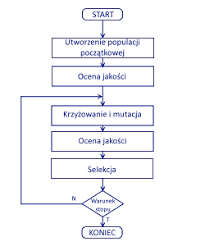
\includegraphics[width=0.6\textwidth]{genetic_pseudocode.png}
        \label{fig:paneloperatorski}
\end{figure}
\newpage
\subsubsection{Uwagi ogólne}
W przypadku tego algorytmu również postanowiliśmy że zrealizujemy dwie wersje tego algorytmu, jednak różniące się jedynie metodą selekcji i krzyżowania. Jako algorytm konstrukcyjny skorzystaliśmy z algorytmu zachłannego. Ustaliśmy również że w każdej generacji wymieniamy wszystkie osobniki, nie uwzględniamy więc przypadku gdy część starszej generacji  pozostaje dostępna w kolejnej (przy czym pozwalamy na przypadek że w wyniku selekcji, krzyżowania i mutacji powstanie identyczny osobnik jak w którejś z poprzednik generacji).
W porównaniu do poprzednich algorytmów dla algorytmów genetycznych musieliśmy zrezygnować z  naszej orginalnej metody symulacji całego gospodarstwa, gdyż doprowadziło by to do niepotrzebnego zwiększenia złożoności obliczeniowej algorytmów. Aby temu zapobiec dla tych podejść postanowiliśmy symulować niezależnie od siebie każde pole z osobna (więc rozwiązaniem algorytmu genetycznego jest wektor roślin dobranych w kolejnych latach do danego pola), w ten sposób w rzeczywistości pojedynczy algorytm genetyczny wykonuje się tyle ile jest pól, jednak dzięki temu podejściu znacznie ułatwiła się końcowa implementacja algorytmu jak i czas trwania algorytmu. Z tego też powodu ostateczny wynik działania algorytmu to suma najlepszych generacji każdego pola.  Uznaliśmy również za rozsądną decyzję by nie udostępniać użytkownikowi zmiany liczbę chromosomów oraz pokoleń które automatycznie dynamicznie dostosowują  się do liczby symulowanych lat i początkowej jakości gleby, zrobiliśmy tak z powodu dość ograniczonej liczby dostępnych roślin i dla pewnych słabszych gleb mogło stać się nie możliwe wylosowanie takiej ilości niepowtarzalnych chromosomów. z uwagi na duże podobieństwo implemetacyhne obu metod poniżej przedstawiamy opis od razu obu podejść:

\subsubsection{Inicjalizacja}
Inicjalizacja wykonuje się tylko raz dla każdego pola w zerowej generacji.
Realizuje ją metoda $initial_result$. Przyjmuje ona początkową generacje, która składa się z zadanej liczby identycznych chromosomów przyjętych z rozwiązania algorytmu zachłannego. Następnie w sposób w każdym z nich podmienia losowy gen, w taki sposób by ostatecznie otrzymać generacje niepowtarzalnych, poprawnych (oraz w razie możliwości dających nie zerowy zysk) osobników.

\subsubsection{Selekcja metoda ruletki}
Po inicjalizacji przechodzimy do etapu selekcji która będzie wykonywała się dla każdej generacji. Realizowana jest ona przez metodę $selection_roulette$. Jako że ta metoda znajduję się na początku każdej generacji uzywamy jej również do sprawdzenia czy nie poprawiła się maksymalna wartość zysku otrzymana w dotychczasowych generacjach. Samą selekcje rozpoczynamy od znalezienia minimalnej wartości zysku w generacji i w przypadku gdy jest ona ujemna  podczas ustalania prawdodopodobieństwa wybrania danego osobnika dodajemy do każdego z nich tą wartość. Robimy tak ponieważ w przypadku ujemnych wartości program dobierał błędne wartości prawdopodobieństw (a w najgorszych przypadkach dochodziło do tego że nie potrafił on dobrać żadnej wartości prawddobieństw). Po owym warunku sumujemy zyski wszystkich chromosomów w generacji, a następnie ustalamy prawdopodobieństwo przyjęcia każdego z osobników, w wyniku dzielenia zysku danego chromosomu przez wyliczoną sumę). Ostatecznie w pętli wybieramy zgodnie z zasadą działania koła ruletki dwójkę rodziców, tak by ostatecznie otrzymać liczbę par równą połowie liczby chromosomów.

\subsubsection{Selekcja metoda rankingowa}
Tak jak dla metody ruletki wykonuje się ona dla każdej generacji oraz sprawdza poprawne najlepszej generacji. Realizuje ją metoda $selection_rank$. Dla tego podejścia początkowo sortujemy osobniki w  generacji a następnie przekazujemy dwa najlepsze chromosomy dalej.
Jest to więc dużo prostsza metoda od względem implementacyjnym dla tego etapu.

\subsubsection{Krzyżowanie metoda ruletki}
Realizowana jest krzyżowanie wielopunktowe przez metode $crossover$ . Dostaje ona rodziców z selekcji następnie dla każdej pary rodziców losujemy zakres genów które następnie są wymieniane między osobnikami rodzicielskimi i w ten sposób powstają osobniki potomne. Przed zwróceniem dzieci następuje jeszcze sprawdzenie czy powstałe osobniki są poprawne.

\subsubsection{Krzyżowanie metoda rank}
Implementacja tego krzyżowania znajduje się w tej samej metodzie co poprzednie krzyżowanie i róźni się jedynie tym że potomstwo tworzone jest jedynie z krzyżowania jednej pary rodziców. Sprowadza się wiec to do wielokrotnego losowania zakresu podmienianych genów dla tej samej pary osobników rodzicielskich.


\subsubsection{Mutacja}
Zaimplemtowana jest w metodzie $mutation$. Otrzymuje ona jako parametr dzieci  które dostaliśmy w wyniku krzyżowania. Do każdego dziecka dodawana jest losowa wartość z zakresu od 0 do 1, a następnie osobniki które otrzymały wartość ponad 0.5 (wartość ta jest zdecydowanie większa niż w większości innych przykładów zastosowania algorytmu genetycznego, jednak z uwagi na dość ograniczoną liczbę możliwości , większość dzieci otrzymana z krzyżowania cechuje się między sobą bardzo małą różnorodnością i zbyt mała prawdopodobność mutacji mogła doprowadzić że algorytm utknął by w minumum lokalnym)  zostaną zmutowane, a pozostałe nie. Wylosowana wartość decyduje również o ilości zmienionych genów. W celu poprawy skuteczności algorytmu owa mutacja dla jednego osobnika jest dokonywana kilka razy i wybierana jest tylko najlepsza mutacja, działanie to nie jest zgodne z ogólnym założeniem algorytmów genetycznych jednak w wyniku testów dla naszego przypadku okazało się że działanie to znacznie poprawia ostateczny wynik. Jako sposobu mutacji skorzystaliśmy z losowej mutacji resetującej dotychczasowe wartośći, więc identycznie jak w inicjalizacji wybieramy rok i zmieniamy związany z nim gen na losowo dobrany inny. Sprawdzamy również czy wylosowany gen nie był już raz zmieniany, jeśli tak to losujemy jeszcze raz. Z uwagi na wpadanie w nieskończoną pętle związaną z narzuconymi ograniczeniami, zastosowaliśmy również licznik ilości takich przekroczeń i jeśli przekroczy on pewną wartość to przywracamy ostatnią poprawną wersję chromosomu i rezygnujemy z dalszej jego modyfikacji.

\subsubsection{Warunek stopu}
Z uwagi że na to że w rzeczywistości algorytm genetyczny wywoływany jest z osobna do każdego pola, które mają różną dynamikę, a przy tym chęcią do wypisywania na wykresie zsumowanych wyników wszytskich pól, uznaliliśmy że nie wprowadzimy warunku stopu zależnego od wyników algorytmu tylko z góry ustalimy liczbę generacji (zależną od liczby lat) po których algorytm się zakończy. Po zakończeniu algorytmu dla jednego pola, najlepszy z osobników zapisywany jest do specjalnej listy która ostatecznie stworzy ostateczną macierz upraw. Na końcu działania całego algorytmu wypisywana jest macierz jakości pól, dokonane wyboru w każdym z roków, oraz numery generacji w których dane pole otrzymało najlepszy wynik.

\section{Aplikacja}
W ramach realizacji naszego projektu zrealizowaliśmy również proste GUI pozwalające w wygodny sposób użytkownikowi korzystać z naszego programu. Aby go uruchomić trzeba mieć pobraną i wypakowaną naszą aplikację, następnie uruchomić $FieldSimulation.exe$ . W ten sposób uruchomi się nam program w okienku oraz konsola. Konsola ta jest tylko do przedstawiania macierzy wynikowych oraz numerów najlepszych generacji z algorytmów genetycznych, jest to więc nie interaktywne narzędzie pomocnicze na które użytkownik nie musi zwracać uwagi jeśli interesują go tylko uzyskany zysk. W wspomnianym już okienku  ustalamy liczbę lat oraz pól które chcemy przesymulować, możemy również wybrać wcześniej przygotowany przypadek domyślny. Jeśli jednak chcemy zadeklarować własne parametry gospodarstwa to klikamy przycisk kontynuuj, wtedy ukazuje się nowe okienko w którym możemy wpisać powierzchnie każdego pola, dystans od gospodarstwa oraz początkową jakość ziemi. Możemy te pola wypełnić samemu lub wylosować, następnie musimy kliknąć ponownie przycisk kontynuuj. Wtedy ukaze nam się ostateczne okno w którym wybieramy jedną z metod symulacji, ustalamy temperature maksymalną dla metody wyżarzania . Możemy tam w górnym prawym rogu obserwować uzyskany zysk dla każdej z metod. Dla metod wyżarzania oraz algorytmów możemy wyświetlić również przebeg rozwiązania za pomocą przycisku w dolnej części okna, ukaże nam się wtedy dodatkowe okienko w którym będziemy mogli dokładnie przyjrzeć się przebiegowi. W  GUI nie udostępniliśmy możliwości zmiany ilości generacji czy liczby chromosomów (powody te opisaliśmy w akapicie dotyczącym algorytmu genetycznego), jeśli jednak użytkownik jest przekonany że chce zmienić te parametry może to zrobić wchodząc w przesłane pliki programu, a następnie otworzyć plik $GUI.py$ i w linijkach 286 oraz 303 powinny znajdować się zmienne ($generation_quantities$ oraz $amount_chromoses$) które decydują o tych parametrach.

\section{testy}
Każdy algorytm został puszczony 10-krotnie (w przypadku wyżarzania dla temperatur 250, 500, 1000)

\subsection{symulowane wyżarzanie ver. 1 - T=250}
Maksymalny zysk : 113 543.61\\
Minimalny zysk: 106 634.53\\
Średni zysk : 109 589.07\\

\begin{figure}[H]
	\centering
	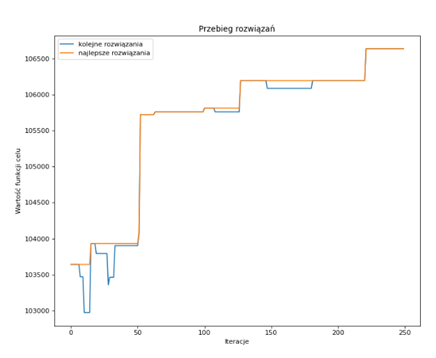
\includegraphics[width=0.7\linewidth]{screens/AnneallingV1_250}
	\caption{Przykładowy wykres rozwiązań dla T = 250}
	\label{fig:anneallingv1250}
\end{figure}


\subsection{symulowane wyżarzanie ver. 1 - T=500}
Maksymalny zysk : 113 435.884\\
Minimalny zysk: 107 481.54\\
Średni zysk : 111 440.51\\

\begin{figure}[H]
	\centering
	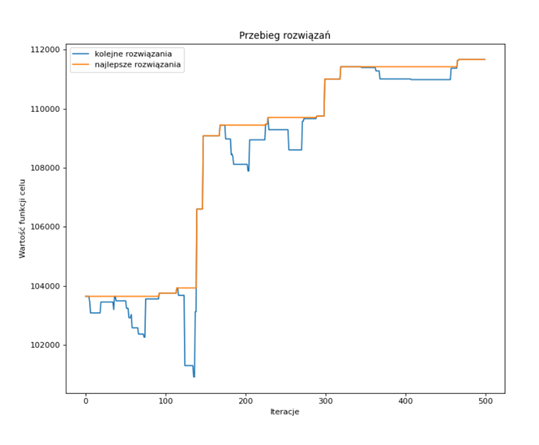
\includegraphics[width=0.7\linewidth]{screens/AnneallingV1_500}
	\caption{Przykładowy wykres rozwiązań dla T = 500}
	\label{fig:anneallingv1500}
\end{figure}


\subsection{symulowane wyżarzanie ver. 1 - T=1000}
Maksymalny zysk : 114 592.91\\
Minimalny zysk: 112 150.77\\
Średni zysk : 113 364.59\\



\begin{figure}[H]
	\centering
	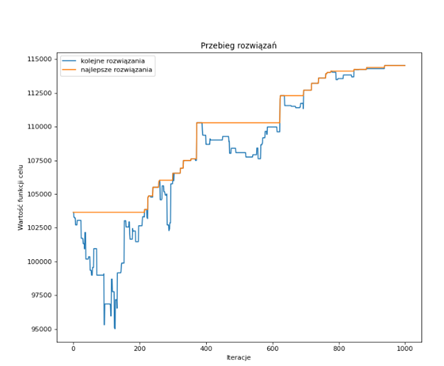
\includegraphics[width=0.7\linewidth]{screens/AnneallingV1_1000}
	\caption{Przykładowy wykres rozwiązań dla T = 1000}
	\label{fig:anneallingv11000}
\end{figure}


\subsection{symulowane wyżarzanie ver. 2 - T=250}
Maksymalny zysk :  113 566.25 \\
Minimalny zysk: 104 620.12 \\
Średni zysk : 107 846.09 \\

\begin{figure}[H]
	\centering
	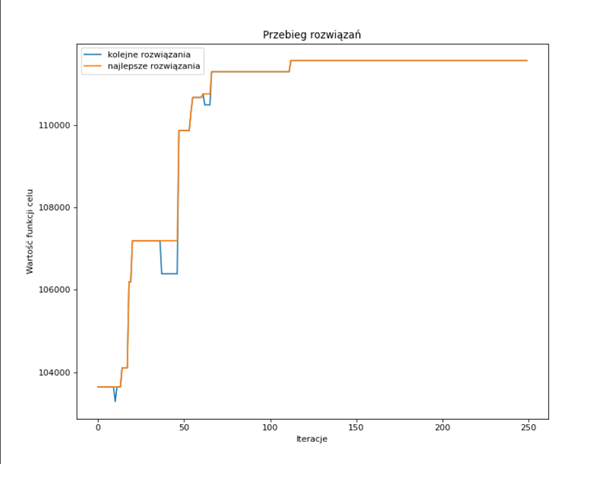
\includegraphics[width=0.7\linewidth]{screens/AnneallingV2_250}
	\caption{Przykładowy wykres rozwiązań dla T = 250}
	\label{fig:anneallingv2250}
\end{figure}


\subsection{symulowane wyżarzanie ver. 2 - T=500}
Maksymalny zysk : 111 502.28 \\
Minimalny zysk: 104 643.50 \\
Średni zysk : 108 609.50 \\

\begin{figure}[H]
	\centering
	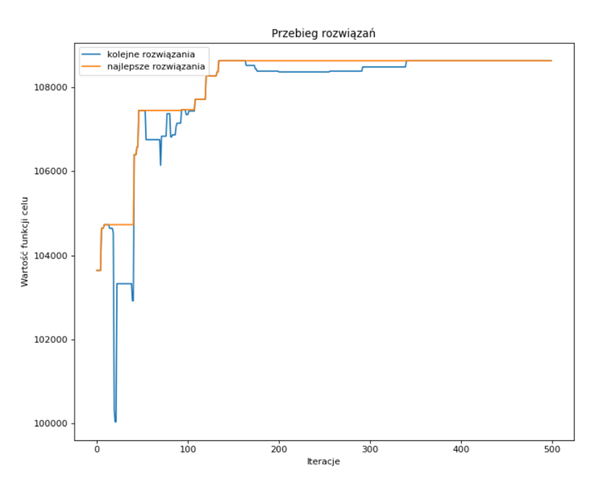
\includegraphics[width=0.7\linewidth]{screens/AnneallingV2_500}
	\caption{Przykładowy wykres rozwiązań dla T = 500}
	\label{fig:anneallingv2500}
\end{figure}


\subsection{symulowane wyżarzanie ver. 2 - T=1000}
Maksymalny zysk : 111 098.25 \\
Minimalny zysk: 103 641.16 \\
Średni zysk : 106 994.41 \\

\begin{figure}[H]
	\centering
	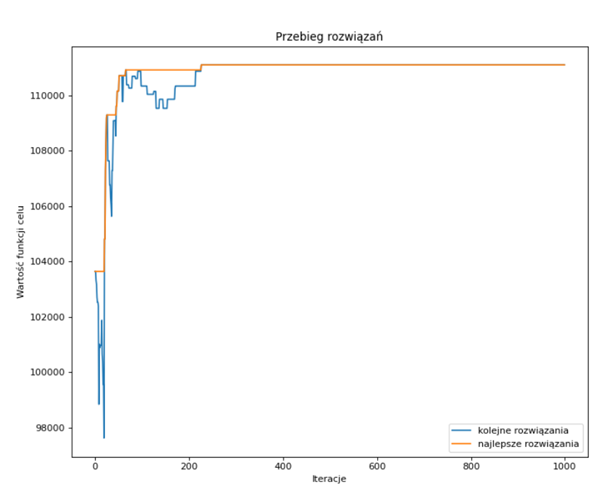
\includegraphics[width=0.7\linewidth]{screens/AnneallingV2_1000}
	\caption{Przykładowy wykres rozwiązań dla T = 1000}
	\label{fig:anneallingv21000}
\end{figure}

\subsection{Genetic algorithm - roulette}
Maksymalny zysk : 115 107.46 \\
Minimalny zysk: 114 060.89 \\
Średni zysk : 114 630.24\\

\begin{figure}[H]
	\centering
	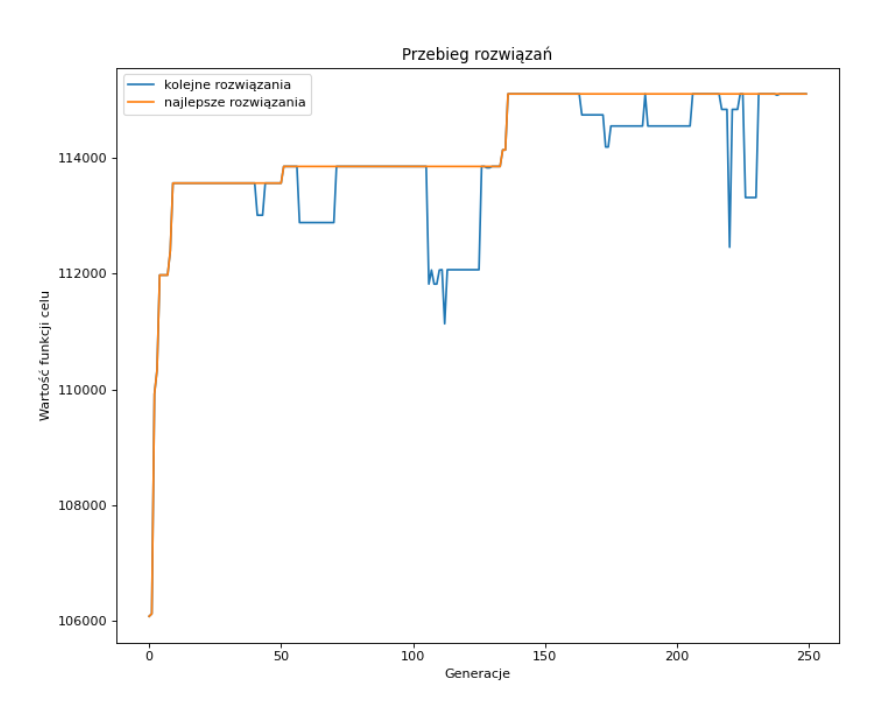
\includegraphics[width=0.7\linewidth]{screens/ruletka}
	\caption{Przykładowy wykres rozwiązań}
	\label{fig:ruletka}
\end{figure}



\subsection{Genetic algorithm - rank selection}
Maksymalny zysk : 115107.46\\
Minimalny zysk: 113 566.25 \\
Średni zysk : 114 665.48\\

\begin{figure}[H]
	\centering
	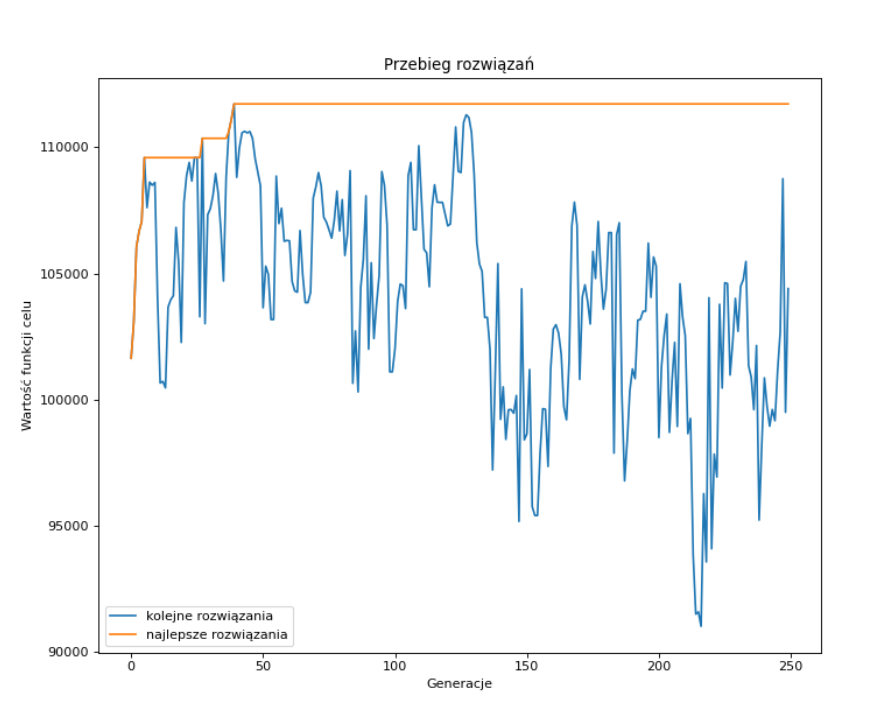
\includegraphics[width=0.7\linewidth]{screens/rank.png}
	\caption{Przykładowy wykres rozwiązań}
	\label{fig:rank}
\end{figure}


\section{Testy - przypadek ze złymi warunkami}

\begin{figure}[H]
	\centering
	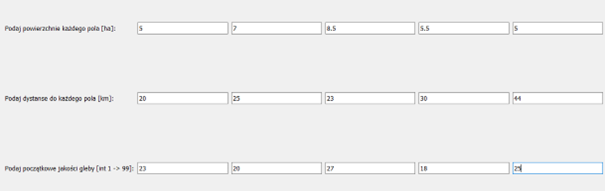
\includegraphics[width=0.7\linewidth]{screens/macierz_zlych_przypadkow}
	\caption{}
	\label{fig:macierzzlychprzypadkow}
\end{figure}


\subsection{annealing v1 - temperatura=1000}
Maksymalny zysk : 75 767.88\\
Minimalny zysk: 59 471.75 \\
Średni zysk : 70 873.31

\begin{figure}[H]
	\centering
	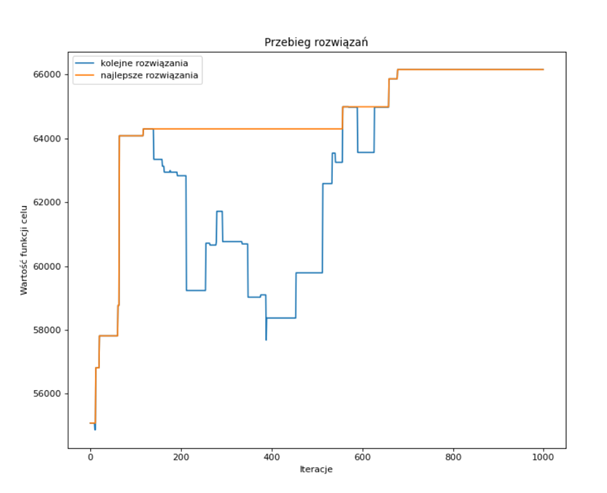
\includegraphics[width=0.7\linewidth]{screens/annealing_v1_zlych_przypadkow}
	\caption{}
	\label{fig:annealingv1zlychprzypadkow}
\end{figure}


\subsection{annealing v2 - temperatura=1000}
Maksymalny zysk : 71 395.16\\
Minimalny zysk: 66 062.65 \\
Średni zysk : 68 839.12

\begin{figure}[H]
	\centering
	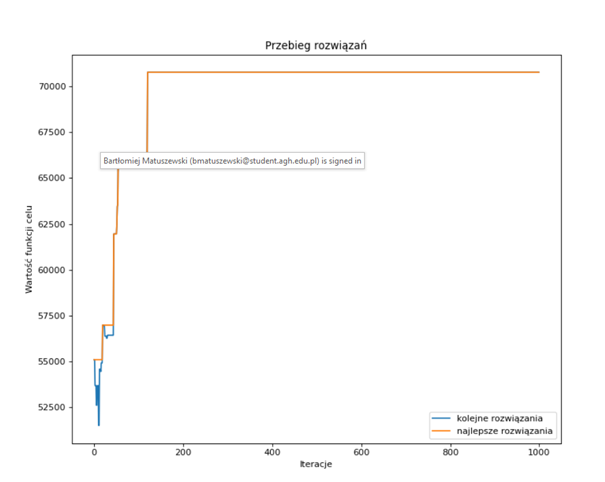
\includegraphics[width=0.7\linewidth]{screens/annealing_v2_zlych_przypadkow}
	\caption{}
	\label{fig:annealingv2zlychprzypadkow}
\end{figure}


\subsection{genetic rank i roulette}

Genetic - rank selection\\
Min: 78 778.63\\
Max: 78 778.63\\
Średnia : 78 778.63\\

\begin{figure}[H]
	\centering
	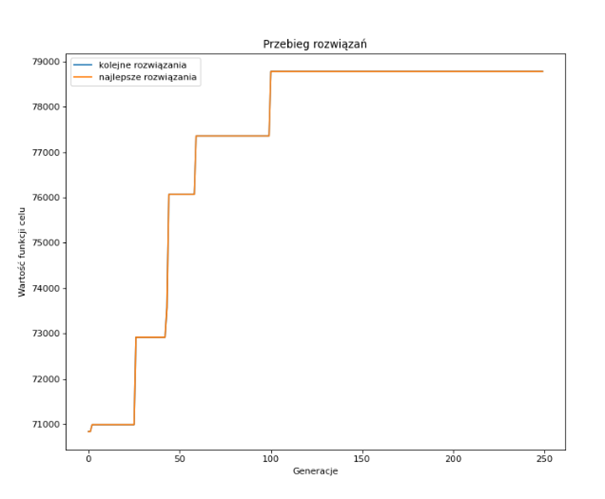
\includegraphics[width=0.7\linewidth]{screens/genetic_rank_zlych_przypadkow}
	\caption{Genetyczny - rankingowy}
	\label{fig:geneticrankzlychprzypadkow}
\end{figure}


Genetic - roulette selection\\
Min: 78 778.63\\
Max: 78 778.63\\
Średnia : 78 778.63\\

\begin{figure}[H]
	\centering
	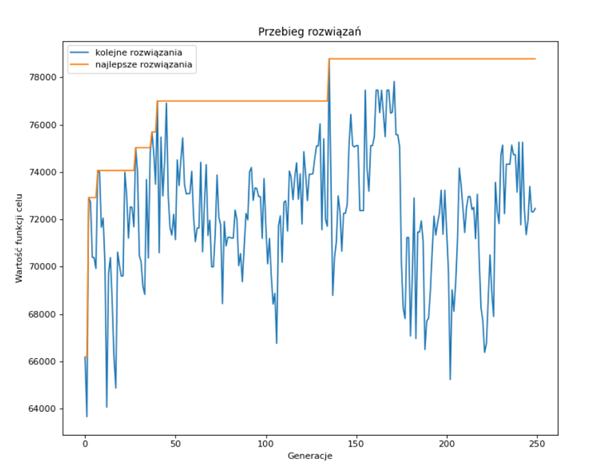
\includegraphics[width=0.7\linewidth]{screens/genetic_roulet_zlych_przypadkow}
	\caption{Genetyczny - ruletkowy}
	\label{fig:geneticrouletzlychprzypadkow}
\end{figure}

Obie wersje genetycznego nie zmieniają wyniku dla takiej macierzy początkowej.


\subsection{greedy}

Min: 55 084.45\\
Max: 55 084.45\\
Średnia : 55 084.45\\

Dla porównania wyniki algorytmu zachłannego




\section{Problemy}
Indeksacja

wybór następnego kandydata na rozwiązanie

źle zaimplementowane dobieranie temperatury (chyba)
\section{Pomysły}
-ograniczyć błąd związany z jakością pola (że jesli w momencie uprawy roślina nie będzie pogorszyć jakości ziemi poniżej zera to można ją puścić)
- możliwość przekazywania części osobników z jednego pokolenia do kolejnego
- możliwość uniknięcia mutacji

\end{document}
